\chapter{Review and Summary}

The human brain is a remarkable and complex organ, and reading is one of its most remarkable capabilities. The small-world organization of the brain is an apparent paradox: to more efficiently integrate disparate functions efficiently, the brain segregates them into smaller modules. Throughout this dissertation, we have investigated the influence of these organizational principles on individual differences in the ability to efficiently integrate brain systems during reading. We combined inferences from several different methodological approaches, including behavioral testing, resting-state network analysis, task-based activation analyses, and the combination of the two. We believe these results represent a contribution to the fields of macro-scale human connectomics, as well to those studying reading and its disabilities.

In the first three studies, we analyzed the network architecture of fourth grade readers under a variety of conditions. Using resting-state networks, we established a set of connectome-forming methods and settled on a set of descriptive metrics including modularity, participation coefficient and path length. Next, we compared individual differences in these attributes to reading skill. We found that better readers had greater global network modularity but reduced modularity in the auditory and cingulo-opercular RSNs, suggesting that this segregated network architecture is important for functioning but that literacy acquisition may impact the composition of specific networks. 

We then sought to describe how network architecture changes \textit{during} reading, and whether task-evoked networks had a different relationship to reading skill than those at rest. In Study 2, we observed that reading comprehension decreased global modularity, especially in the visual, dorsal attention and default mode networks. Overall, it increased measures of integration between a wide-variety of RSNs, including sensory and attention systems. Furthermore, the positive relationship between reading skill and global modularity persisted during comprehension, suggesting that the maintenance of each module across tasks is an important attribute of an efficient connectome. 

Does that mean that \textit{more} similarity between task-evoked network architectures is indicative of a more efficient organization? If so, do some RSNs become more similar and other nodes less so?  To answer these questions, Study 3 compared two related but different processes - reading and listening. We found that there was a common core of areas activated in the two network states, as well as a common network backbone. In fact, better readers had a greater degree of similarity between the two language conditions, suggesting that the two networks merge in more skilled readers. We then calculated network flexibility across many different architectures, including simple attention tasks and rest and found that the listening-to-reading similarity was not unique to language, but inherent to the individual: participants were generally more similar to themselves in different tasks than to others in the same task.

Finally, we investigated the effects of development on modularity and network organization. In Study 4, we replicated previous findings of a relationship between modularity and reading skill in younger readers using novel stimuli and a larger group size. We found that the modular organization of the brain -- as determined by using a group average reference parcellation -- decreases slightly throughout the lifespan but is similarly disrupted during tasks, no matter the age or expertise of the individual. We also identified developmental shifts in network connectivity which show that an emphasis on sensorimotor and dorsal attention systems gives way to connectivity between default mode, auditory, ventral attention and salience systems. Adults also showed greater differences between each other than children did, although their within-subject ``flexibility'' did not change.

\begin{table}[t]
	\renewcommand{\tabcolsep}{0.2cm}
	\centering
	\begin{tabular}{c|p{10cm}}
\toprule 
Figure & Key Finding \\ 
\midrule 
\ref{fig:ch2-global-glm-covariates-thresh} & Global modularity was the graph theory measurement most predictive of reading skill. \\ 
 \ref{fig:ch2-rsn-node-modularity-corr} & Modularity in the auditory and cingulo-opercular networks was anti-correlated with reading skill.	\\ 
\ref{fig:ch3-reading-connectome-activations} & Reading comprehension induces system-level increases in the ventral attention, visual, somatomotor (mouth) and default mode networks.	 \\ 
\ref{fig:ch3-comprehension-reorganization}  & Reading is especially characterized by decreased connectivity \textit{within} sensory, dorsal attention and default mode and increased connectivity \textit{between} many different RSNs.  \\ 
\ref{fig:ch3-modularity-reading-by-condition}  & The positive relationship between network modularity and reading persists during reading comprehension.  \\ 
\ref{fig:ch4-modality-graph-theory}  & Reading comprehension requires more more integration across networks than listening. \\ 
\ref{fig:ch4-modality-similarity-to-reading} & Better readers have greater similarity between their listening and reading networks.
\bottomrule 
\end{tabular}
	\caption[Key findings in Studies 1 through 4.]{Key findings in Studies 1 through 4.}
	\label{table:ch6-key-findings}
\end{table}

Taken as a whole, the studies underscore the importance of functional network architecture in cognitive processing, as well as its stability over time and cognitive states. The results support a neurocognitive model in which efficiently segregated processes serve as a scaffolding for their integration into more complex functions, and over time, the development of new connections and displacement of others individuates each person's connectome. The studies illustrate how a connectomics approach to reading illuminates -- not displaces -- previous neuroimaging research, much of which focused on localizing specific cognitive processes. We made every attempt to be systematic in our methodology, and believe we have made a meaningful contribution to our understanding brain modularity as it relates to cognitive processing. However, there is much left to be investigated, and many possible future directions for these research aims. Below, we outline a few of these.

\section{The attention networks in reading}

One of the consistent findings across our studies was the engagement and disengagement of attentional RSNs in reading. The ventral attention network was the RSN most engaged by reading in Study 2, and the dorsal attention network was one of the only RSNs to show lower activation in reading than in listening (Study 3). Furthermore, adults had greater connectivity between the ventral attention network and many other networks, wheras children had higher modularity with the dorsal attention network and higher connectivity between it and visual and somatosensory systems. Although it's widely recognized that reading relies heavily on attention (e.g. \citep{Vogel2012, Vidyasagar2010, Clifton2016}, it may warrant an even closer relationship to ``language'' processes than it currently bears. Popular models such as the Simple View of Reading, for example, don't account for attention explicitly, instead modeling reading ability as the product of word recognition and oral language comprehension \citep{Gough1988}. 

One of the major benefits of investigating attentional process in reading as opposed to traditional linguistic process is the potential for identifying similarities across multiple cognitive processes. As we have seen, from a network standpoint, the reading network is less unique than might be expected. Apart from a few remarkable regions (the visual word form area, temporo-parietal junction), a great degree of the reading process appears to be the orchestration of pre-existing and highly efficient sensory processes, and attentional networks are key to this orchestration: they will help identify salient words in a large block of text, suppress environmental distractions and maintain focus for extended periods of time \citep{Fedorenko2014}. Slow or inadequately rapid attention-shifting could undermine fluent reading by causing temporal-spatial misalignment in processing, e.g. letter sequence and arrangement \citep{Lallier2009}. Attentional issues such as these could affect performance in other cognitive domains such as specific language impairment and attention deficit / hyperactivity disorder, which frequently have comorbidity with reading disorders \citep{Pennington2006, Margari2013}. One question ripe for investigation is how the push-pull relationship between the dorsal and ventral attention networks proceeds during reading, and whether it varies at different points during the comprehension process. Methods for modelling this question are described in the next section.


\section{Dynamic modeling of network activity}

Brain networks are not static, even though they are often modelled as such. Connectivity patterns are constantly shifting, and changes in the configuration of networks across time (so-called dynamic connectivity) have become an increasingly important domain of research in the past several years. Work using sliding time windows have illustrated that during rest modules alternate between time periods of higher and lower levels of integration (e.g. global efficiency) over time \citep{Zalesky2014}. These changes are periodic and can be consistent throughout different parts of the brain \citep{Handwerker2012}. (See Figure \ref{fig:ch6-dynamic-connectivity} for an example.) Modelling this variability across subjects can be a challenge, since subjects states tend not to be locked in time with each other outside of tasks; however, many advances have been had by using wavelets and other techniques \citep{Zalesky2014}. 

\begin{figure}[t]
	\centering
	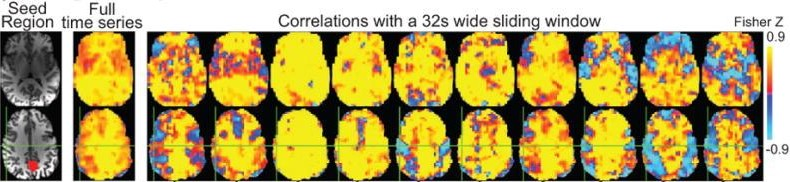
\includegraphics[width=6in]{ch6-dynamic-connectivity}
	\caption[Correlations between brain regions fluctuate over time.]{Correlations between brain regions fluctuate over time. The above figure shows, from left to right: the posterior cingulate seed region; the correlation map created from the seed using a 10 minute time series; correlation maps created over 32s temporal windows. The shorter correlation windows show how functional connectivity changes over time. The authors were able to parse brain regions based on the temporal frequency of these changes in connectivity \citep{Handwerker2012}.}
	\label{fig:ch6-dynamic-connectivity}
\end{figure}

However, answering this question is crucial to understanding our findings of high modularity in better readers. The networks collected were averaged over a relatively long time period -- the course of a few minutes. In that time, there could have been many transitions between low- and high-modularity states. The frequencies at which the brain cycles through these states could be driving the ``average'' global modularity observed in our studies \citep{Fries2005}. Indeed, this oscillatory activity has been the subject of a numbe of studies and represents a promising new dimension to resting-state fMRI analyses \citep{Hutchison2013}. One intersection that these dynamics may address is the ubiquitous role of the default mode network across a number of tasks. In reading, for example, large portions of both the default mode and fronto-parietal networks are active, despite the well-established anti-correlation between them. One explanation could be that some areas of the default mode network oscillate at higher frequencies in order to integrate information into the global workspace \citep{Vatansever2015}.

Another major question relates to the effects of task-switching during reading. Previous research demonstrating the flexibility of the fronto-parietal network in cognition used event-related connectivity measures in which subjectsa task with rapid changes in instructions or event-related working memory tasks \citep{Cole2013, Braun2015}. The FPN may thus be critical for the initial switching action in connectivity patterns, after which the network becomes more settled. In the context of reading, individuals will spend time in various stages of the comprehension process: at some point extra attention will be paid to the decoding of the text, at others to the semantic processing, at others to the recall and integration of previous information \citep{Spreng2013}. Looking at the variations in activity at key junctures of the reading task would elucidate the roles of individual RSNs such as the FPN in the construction, maintenance and evaluation of the text \citep{Sakai2008}. The answers would help to identify whether the ``flexibility'' of certain RSNs and connections are an attribute of that connection or of the task.

\section{Individualized network assignments}

One caveat with connectomics analyses, including those presented here, are that results for the modularity analyses are often based on RSN parcellations from previous literature (e.g. \citep{Power2011}) and are applied indiscriminately across the entire group. This allows for a common reference partition and more interpretable results, but it neglects the fact that there may be important differences between individuals in the optimal community partition for an individual. Even within a given method, there can be a very large number of alternative community parcellations that may differ from the maximum in only a very slight way \citep{Good2010}. Community-agnostic measurements such as the intersection of the union, which we employed in the present analyses, or consensus-based clustering, such as that used in \citep{Power2011}, can address some of these concerns, but is still essentially limited in its ability to allow variability of possible partitions in to the system. 

\begin{figure}[t]
	\centering
	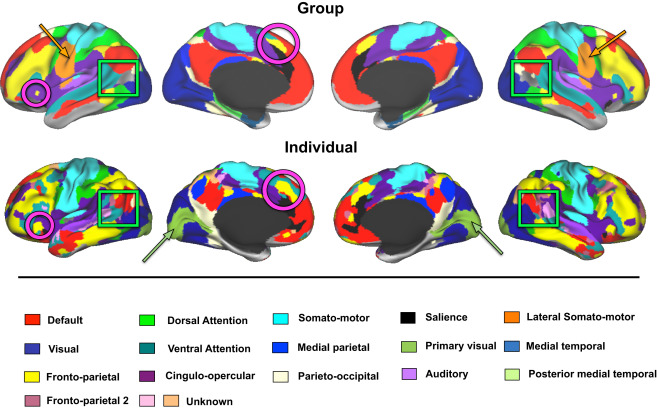
\includegraphics[width=6in]{ch6-individual-parcellation}
	\caption[Individualized networks in a highly sampled individual brain.]{Individualized networks in a highly sampled individual brain. Although the individual's systems-level organization is broadly similar to the group, it demonstrates distinct network features. Figure from \citep{Laumann2015}.}
	\label{fig:ch6-individual-parcellation}
\end{figure}

The problem may be especially acute in the context of development. As we noted in Study 4, as children mature, the pattern of connectivity changes significantly, with modules becoming more segregated and long-range RSNs such as the fronto-parietal network becoming more robustly connected \citep{Cao2016}. In cases where there are actual differences in the architecture, comparison to the same reference partition will result in one group being considered lower modularity when in fact they are more appropriately deemed \textit{different} modularity. One alternative methodology is to create a group average map for each group then assign communities (e.g. \citep{Chan2014}), but as we have seen, this neglects individual differences in the network architecture that may be important and interesting. One important way this can be controlled is by modelling subject's networks on an individual basis and measuring changes longitudinally, as in \citep{Bassett2015}. This allows for the accommodation of individual differences as well the condition effect.


\section{High-resolution and multi-modal parcellations}

One tension present in network analysis is that of resolution: using too coarse of a sampling of the brain and one risks losing important detail; too fine and one risks introducing extra noise and unneeded complexity. In these analyses we used 264 nodes that have been used in a number of other studies (e.g. \citep{Power2013, Cole2014}). These nodes cover a large range of brain systems and functional subdivisions (defined by meta-analytic techniques), and each node is separated by at least 10 mm, meaning there is less redundant information being measured. Functional MRI, however, represents only a narrow sliver of the possible methods for understanding the network architecture of the brain, and how it differs between individuals. Functional methods for human brain mapping can also be found in electroencephalography and magnetoencephalography, which offer much higher temporal resolution. Other whole-brain methods in MRI include white matter tractography and structural covariance. (See \citep{Sui2012} for a review of methods connecting different modalities.) In recent years, the combination of these techniques has resulted in a renaissance of brain mapping, and its impact is beginning to extend into the cognitive domain. 

One of the more influential parcellations has been one developed by Glasser and colleagues using Human Connectome Project data \citep{Glasser2016}. This parcellation utilizes changes in cortical architecture, function, structural connectivity, and topography to delineate 180 cortical areas on each hemisphere of the brain. This large number of areas, and the amount of data it is built on, stands in stark contrast to the 52 Brodmann areas which have long formed the standard schema for analysis. However, this is hardly the only contender: there is also the multimodal Brainnetome (210 parcels), \citep{Fan2016}, Gordon atlas (356) \citep{Gordon2016}, Shen atlas (213) \citep{Shen2013}, and the ubiquitous Yeo (98), Brodman (77) and AAL (74) atlases, among others. 

\begin{figure}[t]
	\centering
	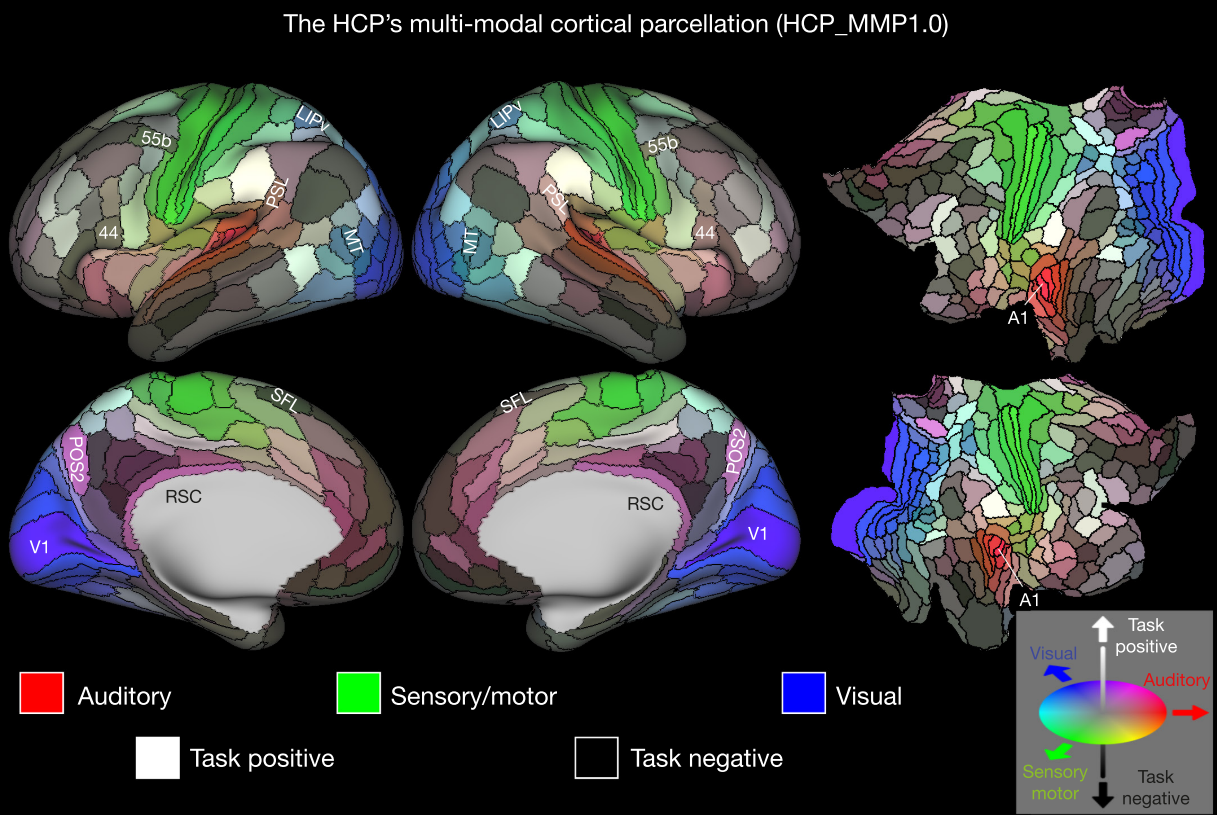
\includegraphics[height=4in]{ch6-multi-modal-parcellation}
	\caption[Multi-modal parcellation of the human brain.]{This high-resolution parcellation of the human brain is based on cortical anatomy, structural tractography and functional covariance. Each hemisphere has 180 regions of interest which can be projected onto a surface map. In this picture, black outlines indicate areal borders and colours indicate the extent to which each area is associated with the corresponding sensorimotor system. Figure from \citep{Glasser2016}.}
	\label{fig:ch6-multi-modal-parcellation}
\end{figure}

The challenges limiting the adoption of these advanced methods -- especially in environments with a more specialized population such as pediatric imaging -- is the amount and quality of data required (multiple modalities, little-to-no subject motion), as well as the steep learning curve associated with implementing them in practice (many pieces of software, advanced programming techniques, many different file types). The number of parcellations can also be overwhelming: although there is a high degree of similarity between each of them, it will be useful for the field to converge on an accepted standard for researchers seeking to bridge the latest advances in network science to their more specific fields. However, as more tutorials become available and software becomes more accessible, future research is likely to reap incredible benefit from these more detailed methods \citep{Poldrack2015}.

\section{Final word}

Reading is a remarkable ability that requires the efficient coordination of information between distributed brain systems. Mastering it is, in John Steinbeck's words, one of ``the most difficult and revolutionary thing that happens to the human brain.'' Why might some children find it easy, even natural, to read, whereas others find it a grueling or impossible chore? One of the great questions in psychology is, what inclines individuals to be different? One piece of the puzzle is likely to be the brain's network architecture: the scaffold developed from the first moments of life through birth and childhood and into adulthood. This architecture provides a scaffold for the ongoing tuning and shaping of the brain, and its efficient organization is important for the myriad cognitive tasks in which people engage, including reading.